% !TEX TS-program = pdflatex
% !TEX encoding = UTF-8 Unicode

\documentclass[11pt]{article}

\usepackage[utf8]{inputenc} % set input encoding (not needed with XeLaTeX)

%%% Examples of Article customizations
% These packages are optional, depending whether you want the features they provide.
% See the LaTeX Companion or other references for full information.

%%% PAGE DIMENSIONS
\usepackage{geometry} % to change the page dimensions
\geometry{a4paper} % or letterpaper (US) or a5paper or....
% \geometry{margin=2in} % for example, change the margins to 2 inches all round
% \geometry{landscape} % set up the page for landscape
%   read geometry.pdf for detailed page layout information

\usepackage{graphicx} % support the \includegraphics command and options

% \usepackage[parfill]{parskip} % Activate to begin paragraphs with an empty line rather than an indent

%%% PACKAGES
\usepackage{booktabs} % for much better looking tables
\usepackage{array} % for better arrays (eg matrices) in maths
\usepackage{paralist} % very flexible & customisable lists (eg. enumerate/itemize, etc.)
\usepackage{verbatim} % adds environment for commenting out blocks of text & for better verbatim
\usepackage{subfig} % make it possible to include more than one captioned figure/table in a single float
\usepackage[hidelinks]{hyperref}
\usepackage{wrapfig} 
\usepackage{suffix} % allows defining commands with *
%\usepackage{showframe} % shows bounding boxes

\usepackage[utf8]{inputenc}
\usepackage[T2A]{fontenc}
\usepackage{hyphenat}
\usepackage[russian]{babel}
\usepackage{mathtools}
\usepackage{amsmath}
\usepackage{amsfonts}

\hyphenation{
наи-мень-ших стер-жня по-лу-чен-но-го бес-ко-неч-ном теп-ло-про-вод-нос-ти тем-пе-ра-ту-ры дол-жен плот-нос-тью ито-го со-от-но-ше-ние па-ра-мет-ра сле-до-ва-тель-но наи-мень-шую пе-ре-се-че-ния най-ти по-лу-чить най-ден-ной тре-бу-ет-ся гра-ви-та-ци-он-но-го по-ло-жим дос-та-точ-но име-ет ри-сун-ка дос-ти-га-ет-ся зна-чит пря-мая ме-тал-ли-чес-ком за-ви-ся-щая по-строй-те под-чи-ня-ет-ся пре-об-ра-зо-ва-ние
}

%%% HEADERS & FOOTERS
\usepackage{fancyhdr} % This should be set AFTER setting up the page geometry
\pagestyle{fancy} % options: empty , plain , fancy
\renewcommand{\headrulewidth}{0pt} % customise the layout...
\lhead{}\chead{}\rhead{}
\lfoot{}\cfoot{\thepage}\rfoot{}

%%% SECTION TITLE APPEARANCE
\usepackage{sectsty}
\allsectionsfont{\sffamily\mdseries\upshape} % (See the fntguide.pdf for font help)
% (This matches ConTeXt defaults)

%%% ToC (table of contents) APPEARANCE2
\usepackage[nottoc,notlof,notlot]{tocbibind} % Put the bibliography in the ToC
\usepackage[titles,subfigure]{tocloft} % Alter the style of the Table of Contents
\renewcommand{\cftsecfont}{\rmfamily\mdseries\upshape}
\renewcommand{\cftsecpagefont}{\rmfamily\mdseries\upshape} % No bold!

\allowdisplaybreaks % automatically wrap lines in math mode

\DeclareMathOperator{\sign}{sgn} % signum - sgn
\newcommand{\Task}[1]{
	\subsection*{\fontfamily{cmss}\selectfont Задача #1.}
	\addcontentsline{toc}{subsection}{Задача #1}
} % task label
\newcommand{\Sln}[1]{
	\subsection*{\fontfamily{cmss}\selectfont Решение.}
	\addcontentsline{toc}{subsection}{Решение задачи #1}
} % solution label
\newcommand{\ScalarProduct}[2]{\langle #1, #2 \rangle} % scalar product
\newcommand{\BigScalarProduct}[2]{\Big \langle #1, #2 \Big \rangle} % scalar product
\newcommand{\Vect}[1]{\mathbf{#1}} % geometric vector
\newcommand{\Fourier}[1]{\mathcal{F} [#1]} % Fourier transform
\newcommand{\bigFourier}[1]{\mathcal{F} \big[ #1 \big]} % Fourier transform for big expressions
\newcommand{\BigFourier}[1]{\mathcal{F} \Big[ #1 \Big]} % Fourier transform for Big expressions
\WithSuffix\newcommand \Fourier*[1]{\mathcal{F}^{-1} [#1]} % inverse Fourier transform
\WithSuffix\newcommand \bigFourier*[1]{\mathcal{F}^{-1} \big[ #1 \big]} % Fourier transform for big expressions
\WithSuffix\newcommand \BigFourier*[1]{\mathcal{F}^{-1} \Big[ #1 \Big]} % Fourier transform for Big expressions
\newcommand{\N}{\mathbb{N}} % Natural numbers - N
\newcommand{\Z}{\mathbb{Z}} % Integer numbers - Z
\newcommand{\Q}{\mathbb{Q}} % Rational numbers - Q
\newcommand{\R}{\mathbb{R}} % Real numbers - R
\newcommand{\Cpx}{\mathbb{C}} % Complex numbers
\newcommand{\e}{\mathrm{e}} % Euler's constant - e
\renewcommand{\d}{\mathrm{d}} % differential - d
\newcommand{\vp}{\operatorname{v. p.}} % principal value - v. p
\newcommand{\erf}{\operatorname{erf}} % error function - erf


\title{Групповой проект по математическому моделированию}
\author{}
\date{}

\begin{document}
\maketitle

\tableofcontents

\section{Решения}

\Task{1} Вслед за лордом Рэлеем найдите период малых колебаний капелек жидкости под действием их поверхностного натяжения, считая, что всё происходит вне гравитационного поля (в космосе).\par

\Sln{1}
Житейкий опыт подсказывает, что период малых колебаний капли должен быть связан с коэффициентом $\sigma$ поверхностного натяжения капли, её плотностью $\rho$ и размером. Поскольку колебания по условию малые, можно считать, что капля имеет объём сферы и её размер вполне описывается радиусом $r$. Итого получаем соотношение
\[ P = f(\sigma, \rho, r). \]

Выпишем размерности введённых величин в системе $L, M, T$:
\begin{equation} \label{eq:eq1}
\begin{split}
[P] & = T^{-1},\\
[\sigma] & = MT^{-2},\\
[\rho] & = ML^{-3},\\
[r] & = L.
\end{split}
\end{equation}

Величины $\sigma, \rho$ и $r$ размерно независимы. Действительно, равенство $\sigma ^\alpha \rho ^\beta r^\gamma =1$ выполняется только при $\alpha = \beta = \gamma = 0$. Значит, для некоторых $p_\sigma, p_\rho, p_r$ и $c_0$ применение $\Pi$-теоремы даёт тождество

\begin{equation} \label{eq:eq2}
\dfrac{P}{\sigma ^{p_\sigma} \rho ^{p_\rho} r^{p_r}} = c_0 
\end{equation}

Так как только $P$ и $\sigma$ выражаются через $T$ (см. (\ref{eq:eq1})), то $p_\sigma = \frac{1}{2}$. Далее, только $\sigma$ и $\rho$ выражаются через 
$M$, а значит, $p_\rho = -p_\sigma = -\frac{1}{2}$. Аналогично находим $p_r = -\frac{3}{2}$. Подставляя найденные числа в (\ref{eq:eq2}), получаем
\[
\dfrac{P}{\sigma ^{\frac{1}{2}} \rho ^{-\frac{1}{2}} r^{-\frac{3}{2}}} = c_0 \iff 
P = c_0 \sqrt{ \dfrac{\sigma}{\rho r^3} }.
\]

\Task{2} В приведённом наборе данных $V$ представляет собой среднюю скорость ходьбы, а $P$ –- численность популяции. Мы хотим узнать, можно ли предсказать численность популяции $P$, наблюдая за тем, как быстро ходят люди. «Подгоните» моделям $P=a \ln V$ и $P=aV^b$ к имеющимся данным с помощью критерия наименьших квадратов. Сравните модели с помощью критерия Фишера.\par

\begin{center}
\begin{tabular}{ |c|c|c|c|c|c|c| }
\hline
$V$ & 4.81 & 4.90 & 5.05 & 5.21 & 5.62 & 5.88\\
\hline
$P$ & 341948 & 49375 & 260200 & 867023 & 1340000 & 1092759\\
\hline
\end{tabular}
\end{center}

\Sln{2}
Сначала подгоним данные к модели $P(V)=a_1\ln V$. Для этого, согласно методу наименьших квадратов, найдём такое $a_1$, что минимизируется значение
\[ \Delta _1 := \sum \limits_{i=1}^n (P_i - a_1 \ln V_i)^2 \]
(в нашем случае всего $n=6$ наборов данных).\par
Для упрощения выкладок рассмотрим векторы $\Vect{p} := (P_1, \ldots, P_n)^\top \in \R^n$ и $\Vect{l} := (\ln V_1, \ldots, \ln V_n)^\top \in \R^n$ (в каноническом базисе). Фиксируем в $\R^n$ стандартное\footnote{Оно даётся формулой $\langle \Vect{x}, \Vect{y} \rangle = x_1 y_1 + \ldots + x_n y_n$, где $\Vect{x} = (x_1, \ldots, x_n)^\top \in \R^n, \Vect{y} = (y_1, \ldots, y_n)^\top \in \R^n$.} евклидово произведение $\langle \cdot, \cdot \rangle$. Тогда верна цепочка
\begin{align*}
\Delta _1 & := \sum \limits_{i=1}^n (P_i - a_1 \ln V_i)^2 =\\
& = \sum \limits_{i=1}^n P_i^2 - 2a_1 \sum \limits_{i=1}^n P_i \ln V_i + a_1^2 \sum \limits_{i=1}^n \ln ^2 V_i =\\
& = \ScalarProduct{\Vect{p}}{\Vect{p}} - 2 \ScalarProduct{\Vect{p}}{\Vect{l}}a_1 + \ScalarProduct{\Vect{l}}{\Vect{l}} a_1^2 = \\
& = \ScalarProduct{\Vect{p}}{\Vect{p}} - \dfrac{\ScalarProduct{\Vect{p}}{\Vect{l}}^2}{\ScalarProduct{\Vect{l}}{\Vect{l}}} +
\ScalarProduct{\Vect{l}}{\Vect{l}} \bigg(  a_1 - \dfrac{\ScalarProduct{\Vect{p}}{\Vect{l}}}{\ScalarProduct{\Vect{l}}{\Vect{l}}} \bigg) ^2 \ge \\
& \ge \ScalarProduct{\Vect{p}}{\Vect{p}} - \dfrac{\ScalarProduct{\Vect{p}}{\Vect{l}}^2}{\ScalarProduct{\Vect{l}}{\Vect{l}}} =\\
& = \dfrac{\ScalarProduct{\Vect{p}}{\Vect{p}}\ScalarProduct{\Vect{l}}{\Vect{l}} - \ScalarProduct{\Vect{p}}{\Vect{l}}^2}{\ScalarProduct{\Vect{l}}{\Vect{l}}} = \min \Delta _1,
\end{align*}
причём наименьшее значение достигается при $a_{1\min}=\ScalarProduct{\Vect{p}}{\Vect{l}} / \ScalarProduct{\Vect{l}}{\Vect{l}}$.\par
В нашем случае $a_{1\min} \approx 408135.750\ldots, \min \Delta _1 \approx 1186996197086.548\ldots$ и 
\[ \chi _1^2 = \sum \limits _{i=1}^6 \dfrac{(P_i - a_{1 \min} \ln V_i)^2}{P(V_i)} \approx 1753774.374\ldots \]

Итак, мы получили зависимость 
\begin{equation} \label{eq:eq3}
P(V) \approx 408135.750 \ln V.
\end{equation}

Займёмся теперь подгонкой данных к модели $P(V)=a_2 V ^{b_2}$. На этот раз требуется оптимизировать величину
\[
\Delta _2 := \sum \limits_{i=1}^n (P_i - a_2 V_i ^{b_2})^2.
\]

Аналогично рассмотрим векторы $\Vect{p} = (P_1, \ldots, P_n)^\top \in \R^n$ и $\Vect{v} = \Vect{v}(b_2) := (V_1^{b_2}, \ldots,\\ V_n^{b_2})^\top \in \R^n, b_2 \in \R$. При каком-нибудь фиксированном $b_2$ оценим $\Delta _2$ снизу по $a_2$ так же, как и в прошлом случае:
\[
\begin{split}
\Delta _2 & := \sum \limits_{i=1}^n (P_i - a_2 V_i ^{b_2})^2 =\\
& = \sum \limits_{i=1}^n P_i^2 - 2a_2 \sum \limits_{i=1}^n P_i V_i^{b_2} + a_2^2 \sum \limits_{i=1}^n V_i^{2 b_2} =\\
& = \ScalarProduct{\Vect{p}}{\Vect{p}} - 2 \ScalarProduct{\Vect{p}}{\Vect{v}}a_2 + \ScalarProduct{\Vect{v}}{\Vect{v}} a_2^2 = \\
& = \ScalarProduct{\Vect{p}}{\Vect{p}} - \dfrac{\ScalarProduct{\Vect{p}}{\Vect{v}}^2}{\ScalarProduct{\Vect{v}}{\Vect{v}}} +
\ScalarProduct{\Vect{v}}{\Vect{v}} \bigg(  a_2 - \dfrac{\ScalarProduct{\Vect{p}}{\Vect{v}}}{\ScalarProduct{\Vect{v}}{\Vect{v}}} \bigg) ^2 \ge \\
& \ge \ScalarProduct{\Vect{p}}{\Vect{p}} - \dfrac{\ScalarProduct{\Vect{p}}{\Vect{v}}^2}{\ScalarProduct{\Vect{v}}{\Vect{v}}} =\\
& = \dfrac{\ScalarProduct{\Vect{p}}{\Vect{p}}\ScalarProduct{\Vect{v}}{\Vect{v}} - \ScalarProduct{\Vect{p}}{\Vect{v}}^2}{\ScalarProduct{\Vect{v}}{\Vect{v}}},
\end{split}
\]
где минимум достигается при $a_{2 \min}=\ScalarProduct{\Vect{p}}{\Vect{v}} / \ScalarProduct{\Vect{v}}{\Vect{v}}$. Полученную функцию от $b_2$ уже можно оптимизировать численными методами, но можно поступить и иначе.\par
Преобразуем последнюю дробь:
\[
\begin{split}
\dfrac{\ScalarProduct{\Vect{p}}{\Vect{p}}\ScalarProduct{\Vect{v}}{\Vect{v}} - \ScalarProduct{\Vect{p}}{\Vect{v}}^2}{\ScalarProduct{\Vect{v}}{\Vect{v}}} & = \dfrac{\ScalarProduct{\Vect{p}}{\Vect{p}}\ScalarProduct{\Vect{v}}{\Vect{v}} - \ScalarProduct{\Vect{p}}{\Vect{v}} \ScalarProduct{\Vect{p}}{\Vect{v}}}{\ScalarProduct{\Vect{v}}{\Vect{v}}}\\
& = \dfrac{\ScalarProduct{\Vect{p}}{\ScalarProduct{\Vect{v}}{\Vect{v}} \Vect{p}} - \ScalarProduct{\Vect{p}}{\ScalarProduct{\Vect{p}}{\Vect{v}} \Vect{v}}}{\ScalarProduct{\Vect{v}}{\Vect{v}}} =\\
& = \dfrac{\ScalarProduct{\Vect{p}}{\ScalarProduct{\Vect{v}}{\Vect{v}} \Vect{p} - \ScalarProduct{\Vect{p}}{\Vect{v}} \Vect{v}}}{\ScalarProduct{\Vect{v}}{\Vect{v}}} =\\
& = \BigScalarProduct{\Vect{p}}{ \dfrac{\ScalarProduct{\Vect{v}}{\Vect{v}}}{\ScalarProduct{\Vect{v}}{\Vect{v}}} \Vect{p} - \dfrac{\ScalarProduct{\Vect{p}}{\Vect{v}}}{\ScalarProduct{\Vect{v}}{\Vect{v}}} \Vect{v} } =\\
& = \BigScalarProduct{\Vect{p}}{ \Vect{p} - \dfrac{\ScalarProduct{\Vect{p}}{\Vect{v}}}{\ScalarProduct{\Vect{v}}{\Vect{v}}} \Vect{v} }.
\end{split}
\]

Нетрудно сообразить, что, каково бы ни было $b_2$, (для данного набора данных) векторы $\Vect{p}$ и $\Vect{v}(b_2)$ неколлинеарны. Значит, их можно ортогонализовать. Применяя алгоритм Грама--Шмидта к системе ($\Vect{v}, \Vect{p}$), получим ортогональную систему ($\Vect{v}, \Vect{s}$), где 

\[
\Vect{s} = \Vect{s}(b_2) = \Vect{p} - \dfrac{\ScalarProduct{\Vect{p}}{\Vect{v}}}{\ScalarProduct{\Vect{v}}{\Vect{v}}} \Vect{v}
\]
--- перпендикуляр к $\Vect{v}$ (рис. \ref{fig:fig-1}).

\begin{figure}[h]
%\vspace{5pt}
\centering
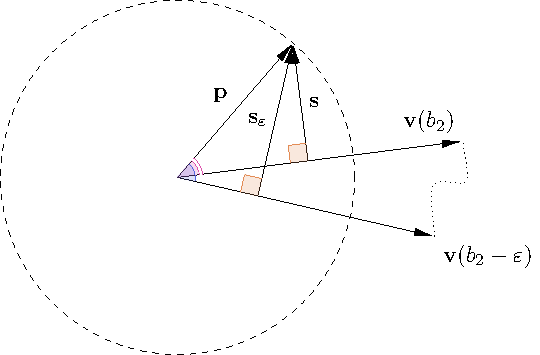
\includegraphics[page=1]{figures.pdf}
\caption{Векторы $\Vect{v}(b_2)$ и $\Vect{s}=\Vect{s}(b_2)$ меняются  с изменением $b_2$.}
\label{fig:fig-1}
%\vspace{5pt}
\end{figure}

Для того чтобы минимизировать значение $\ScalarProduct{\Vect{p}}{\Vect{s}}$, требуется увеличить угол $\angle (\Vect{p}, \Vect{s})$ и уменьшить $\lVert \Vect{s}\rVert$, а для этого (см. рис. \ref{fig:fig-1}) необходимо и достаточно уменьшить
\[
\angle (\Vect{p}, \Vect{v}) = \arccos \bigg\{ \dfrac{\ScalarProduct{\Vect{p}}{\Vect{v}}}{ \sqrt{\ScalarProduct{\Vect{p}}{\Vect{p}}\ScalarProduct{\Vect{v}}{\Vect{v}}} } \bigg\}.
\]
Значит, $\Delta _2$ минимизируется при том же $b_2$, при котором максимизируется значение
\[
\bigg( \dfrac{\ScalarProduct{\Vect{p}}{\Vect{v}(b_2)}}{ \sqrt{\ScalarProduct{\Vect{p}}{\Vect{p}}\ScalarProduct{\Vect{v}(b_2)}{\Vect{v}(b_2)}} } \bigg)^2 =  \dfrac{\ScalarProduct{\Vect{p}}{\Vect{v}(b_2)}^2}{ \ScalarProduct{\Vect{p}}{\Vect{p}}\ScalarProduct{\Vect{v}(b_2)}{\Vect{v}(b_2)} }.
\]

В ходе численного решения были последовательно найдены числа
\[ b_{2 \min} \approx 6.888\ldots, a_{2 \min} \approx  6.651\ldots, \min \Delta _2 \approx 424800366918.064\ldots \]
и
\[ \chi _2^2 = \sum \limits _{i=1}^6 \dfrac{(P_i - a_{2 \min} V_i^{b_{2 \min}})^2}{P(V_i)} \approx 703550.381\ldots \]

Значит, искомая зависимость имеет вид
\begin{equation} \label{eq:eq4}
P(V) \approx 6.651 V^{6.888}.
\end{equation}

Сравним полученные модели (\ref{eq:eq3}) и (\ref{eq:eq4}):
\[
\dfrac{\chi _2^2}{\chi _1^2} \approx 40\%.
\]

Найденные зависимости изображены на рисунке \ref{fig:fig-2}:

\begin{figure}[h]
%\vspace{5pt}
\centering
\includegraphics[page=2]{figures.pdf}
\caption{Сравнение полученных моделей}
\label{fig:fig-2}
%\vspace{5pt}
\end{figure}

\Task{3} Изучается распределение температуры $u=u(x, t)$ в тонком бесконечном металлическом стержне, боковая поверхность которого теплоизолирована. Внутри стержня нет источника тепла. Коэффициент температуропроводности стержня $\alpha^2 = \frac{1}{20}$. Начальное распределение температуры в стержне имеет вид
\[
\varphi (x)=(1-x)(\theta (x)- \theta (x-1)),
\]
где 
\[
\theta (x) =
\begin{cases}
0, x < 0,\\
1, x \ge 0
\end{cases}
\]
--- ступенчатая функция Хевисайда.\\

 \begin{enumerate}
\item Решите задачу с помощью преобразования Фурье и постройте 3D-график полученного решения.
\item Постройте анимацию пространственно-временного распределения температуры в стержне при $0 \le t \le 5$.
\end{enumerate}

\Sln{3}
Начально-кравевая задача для $u=u(x, t)$ имеет вид

\begin{equation} \label{eq:eq5}
\begin{cases}

\displaystyle
\dfrac{\partial u}{\partial t} - \alpha ^2 \dfrac{\partial ^2 u}{\partial x^2} = 0,\\
u(x, 0) = \varphi (x).

\end{cases}
\end{equation}
(Первое уравнение системы, очевидно, является уравнением теплопроводности стержня.)\par
Обозначим соответственно через $U = U_y (t) := \Fourier{u}(y, t)$ и $\Phi (y) := \Fourier{\varphi}(y)$ преобразования Фурье по первому аргументу функций $u$ и $\varphi$. С учётом того, что для всяких чисел $k \in \N$ и $\mu, \nu \in \Cpx$ и любых абсолютно интегрируемых на $\R$ функций $f, g$ 
\[
\begin{split}
& \BigFourier{ \dfrac{\partial u}{\partial t} }(y, t) = \dfrac{\partial}{\partial t} \Fourier{u}(y, t) = \dfrac{\d U}{\d t} = \dot{U},\\
& \BigFourier{ \dfrac{\partial ^k u}{\partial x^k} }(y, t)  = (iy)^k \Fourier{u}(y, t) = (iy)^k U,\\
& \Fourier{\mu f + \nu g} = \mu \Fourier{f} + \nu \Fourier{g},
\end{split}
\]
система (\ref{eq:eq5})  примет вид задачи Коши:

\begin{equation} \label{eq:eq6}
\begin{cases}
\displaystyle
\dot{U} + \alpha ^2 y^2 U = 0,\\
U(0) = \Phi (y).
\end{cases}
\end{equation}
Легко видеть, что её решеним является функция $U_y (t) = \Phi (y) \e ^{-\alpha ^2 y^2 t}$. Чтобы получить решение $u(x, t)$ исходной задачи, найдём обратное преобразование Фурье к данному решению:
\[
\begin{split}
\displaystyle
u(x, t) & = \Fourier*{U_y} = \Fourier*{\Phi (y) \e ^{-\alpha ^2 y^2 t}} =\\
& = \Fourier*{\Phi} * \Fourier*{\e ^{-\alpha ^2 y^2 t}} =\\
& = \varphi (s) * \dfrac{\exp \bigg\{ -\dfrac{s^2}{4\alpha ^2 t} \bigg\}}{\sqrt{2t} \alpha} =\\
& = \dfrac{1}{\sqrt{2 \pi}} \int \limits _{-\infty}^\infty \varphi (s) \dfrac{\exp \bigg\{ -\dfrac{(x-s)^2}{4\alpha ^2 t} \bigg\}}{\sqrt{2t} \alpha} \d s,
\end{split}
\]
где интеграл понимается в смысле главного значения. В выкладке использовалось то, что
\[
\begin{split}
& \Fourier*{f \cdot g} = \Fourier*{f} * \Fourier*{g},\\
& \bigFourier*{\e ^{-\nu ^2 y^2}} = \dfrac{\e ^ {-\frac{x^2}{4\nu ^2}}}{\sqrt{2} \nu}.\\
\end{split}
\]

Вычислим последний интеграл. Для начала заметим, что
\[
\varphi (s)=(1-s)(\theta (s)- \theta (s-1)) =
\begin{cases}
1-s, 0 \le s \le 1,\\
0, s \in \R \backslash [0, 1].
\end{cases}
\]
В таком случае
\begin{align*}
\dfrac{1}{\sqrt{2 \pi}} & \int \limits _{-\infty}^\infty \varphi (s) \dfrac{\exp \bigg\{ -\dfrac{(x-s)^2}{4\alpha ^2 t} \bigg\}}{\sqrt{2t} \alpha} \d s =
\dfrac{1}{2\alpha \sqrt{\pi t}} \int \limits _0^1 (1-s) \exp \bigg\{ -\dfrac{(x-s)^2}{4\alpha ^2 t} \bigg\} \d s =\\
& = \dfrac{1}{2\alpha \sqrt{\pi t}} \int \limits _0^1 \big( (1-x)+(x-s) \big) \exp \bigg\{ -\dfrac{(x-s)^2}{4\alpha ^2 t} \bigg\} \d s =\\
& = \dfrac{1-x}{2\alpha \sqrt{\pi t}} \int \limits _0^1 \exp \bigg\{ -\dfrac{(x-s)^2}{4\alpha ^2 t} \bigg\} \d s \ + \dfrac{1}{2\alpha \sqrt{\pi t}} \int \limits _0^1 (x-s) \exp \bigg\{ -\dfrac{(x-s)^2}{4\alpha ^2 t} \bigg\} \d s =\\
& = \dfrac{1-x}{2} \bigg[ \erf \bigg( \dfrac{x}{2\alpha \sqrt{t}} \bigg) - \erf \bigg( \dfrac{x-1}{2\alpha \sqrt{t}} \bigg) \bigg] -\\
& - \alpha \sqrt{ \dfrac{t}{\pi} } \bigg[ \exp \bigg( -\dfrac{x^2}{4\alpha ^2 t} \bigg) - \exp \bigg( -\dfrac{(x-1)^2}{4\alpha ^2 t} \bigg)  \bigg].
\end{align*}


Итак, окончательно
\begin{align*}
u(x, t) = \dfrac{1-x}{2} \bigg[ \erf \bigg( \dfrac{x}{2\alpha \sqrt{t}} \bigg) & - \erf \bigg( \dfrac{x-1}{2\alpha \sqrt{t}} \bigg) \bigg] -\\
& - \alpha \sqrt{ \dfrac{t}{\pi} } \bigg[ \exp \bigg( -\dfrac{x^2}{4\alpha ^2 t} \bigg) - \exp \bigg( -\dfrac{(x-1)^2}{4\alpha ^2 t} \bigg)  \bigg].
\end{align*}

Как видно, полученная функция не определена при $t=0$. Однако изначально она удовлетворяла тождеству $u(x, t) = \Fourier*{\Phi (y) \e ^{-\alpha ^2 y^2 t}}$, поэтому $u(x, 0) = \Fourier*{\Phi (y)} = \varphi (x)$. Вспоминая, что $\alpha ^2 = \frac{1}{20}$, запишем ответ:
\[
u(x, t) =
\begin{cases}

\begin{split}
\dfrac{1-x}{2} \bigg[ \erf & \bigg( \sqrt{ \dfrac{5}{t} } x \bigg) - \erf \bigg( \sqrt{ \dfrac{5}{t} }(x-1) \bigg) \bigg] -\\
& - \sqrt{ \dfrac{t}{20\pi} } \bigg[ \exp \bigg( -\dfrac{5x^2}{t} \bigg) - \exp \bigg( -\dfrac{5(x-1)^2}{t} \bigg)  \bigg]\ \text{при}\ t > 0,
\end{split}
\\
\varphi (x)\ \text{при}\ t = 0.

\end{cases}
\]

\Task{4} Максимизируйте целевую функцию $g(x, y)=2x-y$ при следующих условиях:
\begin{equation} \label{eq:eq7}\tag{M}
\begin{cases}
x \le 3,\\
y \ge -1,\\
-2x-3y \le 6,\\
-x+2y \le 6.
\end{cases}
\end{equation}

\begin{wrapfigure}{o}{0.6\textwidth}
\centering
\includegraphics[page=3]{figures.pdf}
\caption{Графическое решение задачи}
\label{fig:fig-3}
\end{wrapfigure}


\Sln{4}
Решим задачу графически. Положим $2x-y=c$ и изобразим на плоскости $xOy$ множество \ref{eq:eq7}. С ростом параметра $c$ прямая $2x-y=c$ опускается вдоль оси ординат, следовательно, достаточно найти такие точки $(x, y)$, при которых прямая $2x-y=c$ пересекает множество \ref{eq:eq7} и имеет наименьшую ординату точки пересечения с осью $Oy$. Из рисунка \ref{fig:fig-3} видно, что это достигается в точке $(3, -1)$, а значит, 
\[
\max_{(x, y) \in M}(2x-y) = 7.
\]


\end{document}






























